%%%%%%%%%1%%%%%%%%%2%%%%%%%%%3%%%%%%%%%4%%%%%%%%%5%%%%%%%%%6%%%%%%%%%7%%%%%%%%%8
% Beamer Header
%%%%%%%%%1%%%%%%%%%2%%%%%%%%%3%%%%%%%%%4%%%%%%%%%5%%%%%%%%%6%%%%%%%%%7%%%%%%%%%8

\documentclass[compress,english]{beamer}
\usetheme{sthlm}

% Basic beamer packages
\usepackage{booktabs}
\usepackage{datetime}
\usepackage{dtklogos}
\usepackage{graphicx}
\usepackage{multicol}
\usepackage{pgfplots}
\usepackage{ragged2e}
\usepackage{tabularx}
\usepackage{tikz}
\usepackage{wasysym}

\pgfplotsset{compat=1.8}

\usepackage[utf8]{inputenc}
\usepackage[T1]{fontenc}
\usepackage{newpxtext,newpxmath}

% tikz
\usepackage{tikz}
\usetikzlibrary{patterns,backgrounds,mindmap}

% additional packages
\usepackage{listings}
\usepackage{units}
\usepackage{babel}
\usepackage{sansmath}

\makeatother

%%%%%%%%%1%%%%%%%%%2%%%%%%%%%3%%%%%%%%%4%%%%%%%%%5%%%%%%%%%6%%%%%%%%%7%%%%%%%%%8
% Graphics Path
%%%%%%%%%1%%%%%%%%%2%%%%%%%%%3%%%%%%%%%4%%%%%%%%%5%%%%%%%%%6%%%%%%%%%7%%%%%%%%%8

\graphicspath{{images/}{../images/}}

%%%%%%%%%1%%%%%%%%%2%%%%%%%%%3%%%%%%%%%4%%%%%%%%%5%%%%%%%%%6%%%%%%%%%7%%%%%%%%%8
% Default Background Image
%%%%%%%%%1%%%%%%%%%2%%%%%%%%%3%%%%%%%%%4%%%%%%%%%5%%%%%%%%%6%%%%%%%%%7%%%%%%%%%8

%\usebackgroundtemplate%
%	{\includegraphics[width=\paperwidth,height=\paperheight]{background2.png}}

%%%%%%%%%1%%%%%%%%%2%%%%%%%%%3%%%%%%%%%4%%%%%%%%%5%%%%%%%%%6%%%%%%%%%7%%%%%%%%%8
% Presentation Information
%%%%%%%%%1%%%%%%%%%2%%%%%%%%%3%%%%%%%%%4%%%%%%%%%5%%%%%%%%%6%%%%%%%%%7%%%%%%%%%8

\title{Notes for 2016 Watershed Forum}
\author{Jeffrey Kantor }
\institute{University of Notre Dame \\ Github: \href{http://jckantor.github.io/Rainy-Lake-Hydrology/}{http://jckantor.github.io/Rainy-Lake-Hydrology/}}
\subtitle{Model predictive control strategies for implementing rule curves for 
          the Namakan Reservoir / Rainy Lake Watershed}
\date{2015 International Rainy-Lake of the Woods Watershed Forum \\ 
      March, 2016}

\begin{document}

%%%%%%%%%1%%%%%%%%%2%%%%%%%%%3%%%%%%%%%4%%%%%%%%%5%%%%%%%%%6%%%%%%%%%7%%%%%%%%%8
% Title Page
%%%%%%%%%1%%%%%%%%%2%%%%%%%%%3%%%%%%%%%4%%%%%%%%%5%%%%%%%%%6%%%%%%%%%7%%%%%%%%%8

\setbeamercolor{title}{fg=blue}
\setbeamercolor{subtitle}{fg=white}
\setbeamercolor{date}{fg=white}
\setbeamercolor{author}{fg=white}
\setbeamercolor{institute}{fg=white}

\setbeamerfont{title}{series=\bfseries}

{\usebackgroundtemplate%
	{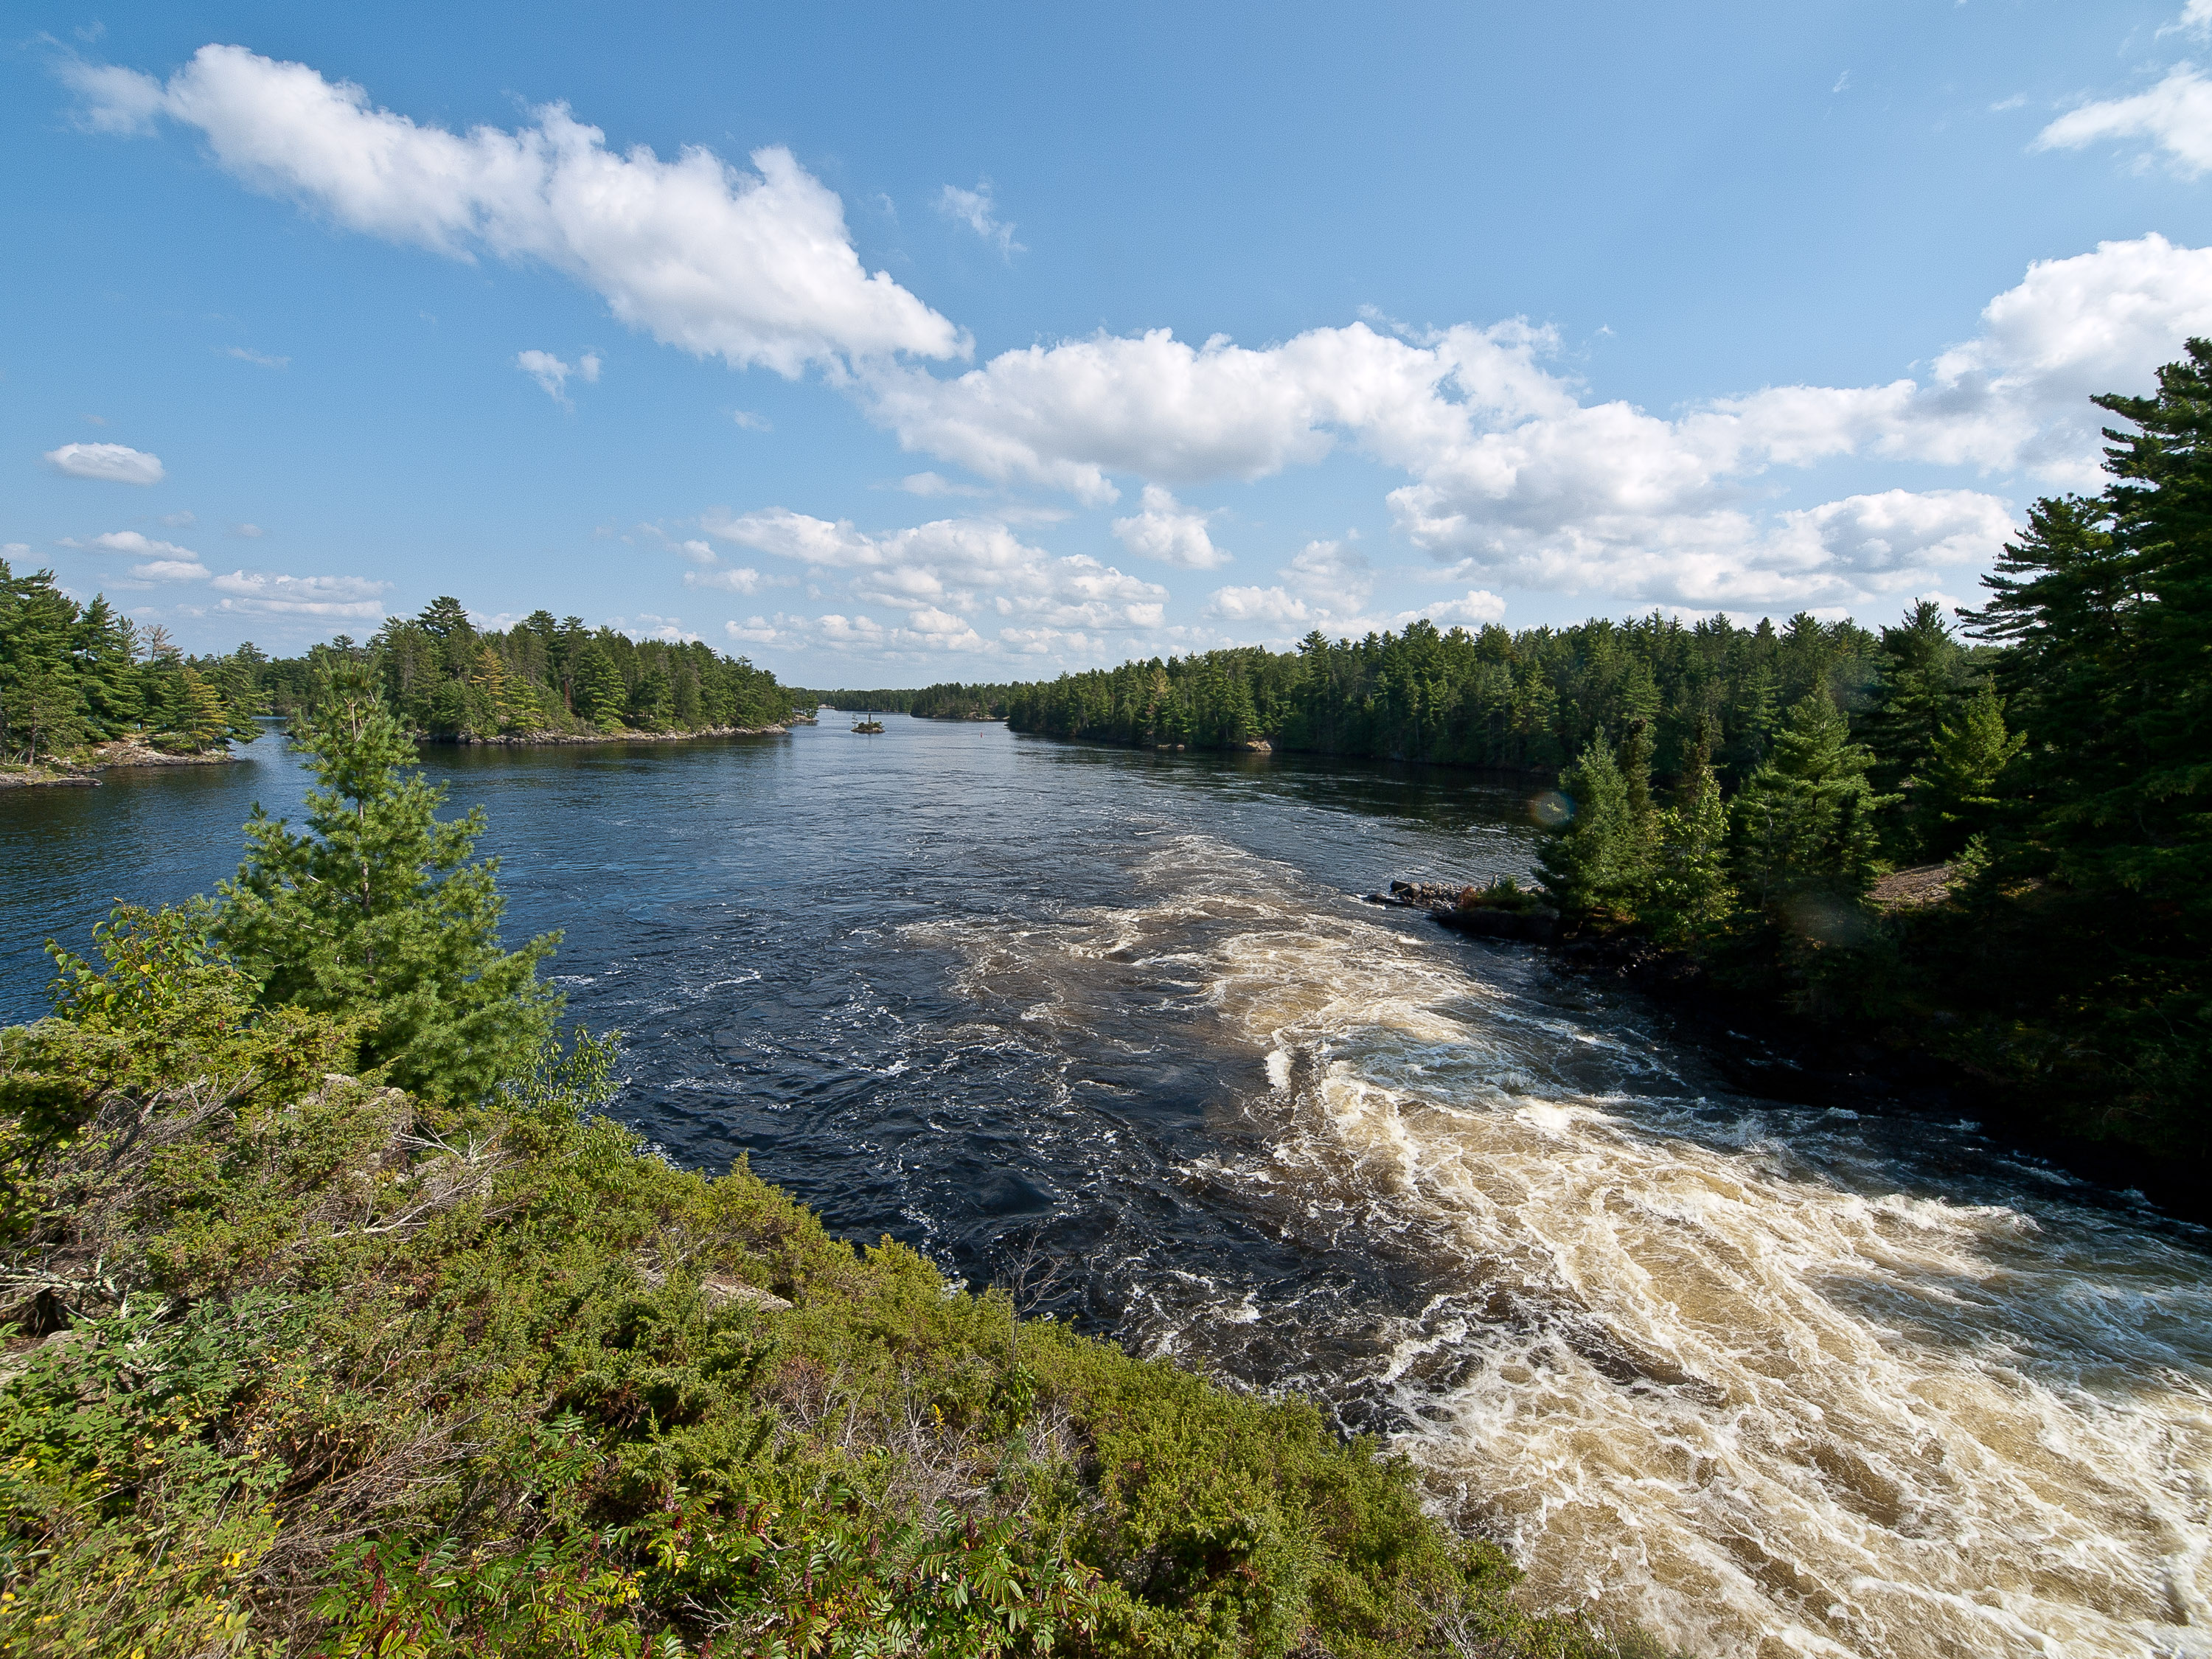
\includegraphics[height=\paperheight]{KettleChannel.jpg}}

\begin{frame}[plain]
\titlepage
\end{frame}
}

%%%%%%%%%1%%%%%%%%%2%%%%%%%%%3%%%%%%%%%4%%%%%%%%%5%%%%%%%%%6%%%%%%%%%7%%%%%%%%%8
% Table of Contents
%%%%%%%%%1%%%%%%%%%2%%%%%%%%%3%%%%%%%%%4%%%%%%%%%5%%%%%%%%%6%%%%%%%%%7%%%%%%%%%8

\section*{Overview}
\begin{frame}{Overview}
% For longer presentations hideallsubsections
\tableofcontents[hideallsubsections]
\end{frame}

%%%%%%%%%1%%%%%%%%%2%%%%%%%%%3%%%%%%%%%4%%%%%%%%%5%%%%%%%%%6%%%%%%%%%7%%%%%%%%%8
% Section 
%%%%%%%%%1%%%%%%%%%2%%%%%%%%%3%%%%%%%%%4%%%%%%%%%5%%%%%%%%%6%%%%%%%%%7%%%%%%%%%8

{\usebackgroundtemplate%
	{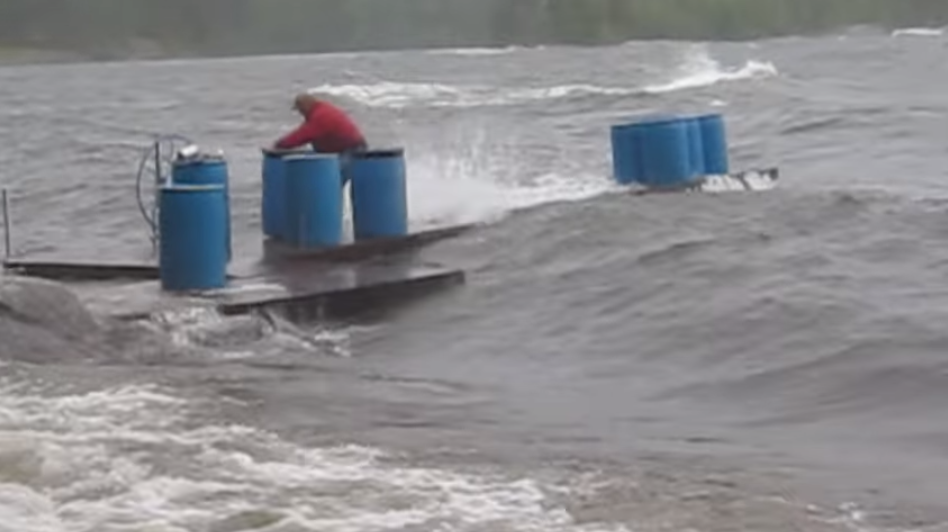
\includegraphics[height=\paperheight]{WaterBarrelsDock}}
\section{Evidence of Climate Change}
}

%%%%%%%%%1%%%%%%%%%2%%%%%%%%%3%%%%%%%%%4%%%%%%%%%5%%%%%%%%%6%%%%%%%%%7%%%%%%%%%8
\begin{frame}{Rainy River Drainage Basin}

\begin{center}
\includegraphicscopyright[width=0.8\paperwidth]{75242923}{Source: International Rainy Lake Board of Control (now IRLWWB)}
\end{center}

\end{frame}

%%%%%%%%%1%%%%%%%%%2%%%%%%%%%3%%%%%%%%%4%%%%%%%%%5%%%%%%%%%6%%%%%%%%%7%%%%%%%%%8
\begin{frame}{Rainy Lake and Namakan Lake Levels 1911--}

Clearly see three rule curve regimes ...
\begin{center}
\includegraphicscopyright[width=0.75\paperwidth]{RainyNamakanLakeLevels.png}{Source: \href{http://jckantor.github.io/Rainy-Lake-Hydrology/}{Github Repository for this paper.}}
\end{center}

\end{frame}


%%%%%%%%%1%%%%%%%%%2%%%%%%%%%3%%%%%%%%%4%%%%%%%%%5%%%%%%%%%6%%%%%%%%%7%%%%%%%%%8
% Section 
%%%%%%%%%1%%%%%%%%%2%%%%%%%%%3%%%%%%%%%4%%%%%%%%%5%%%%%%%%%6%%%%%%%%%7%%%%%%%%%8

{\usebackgroundtemplate%
	{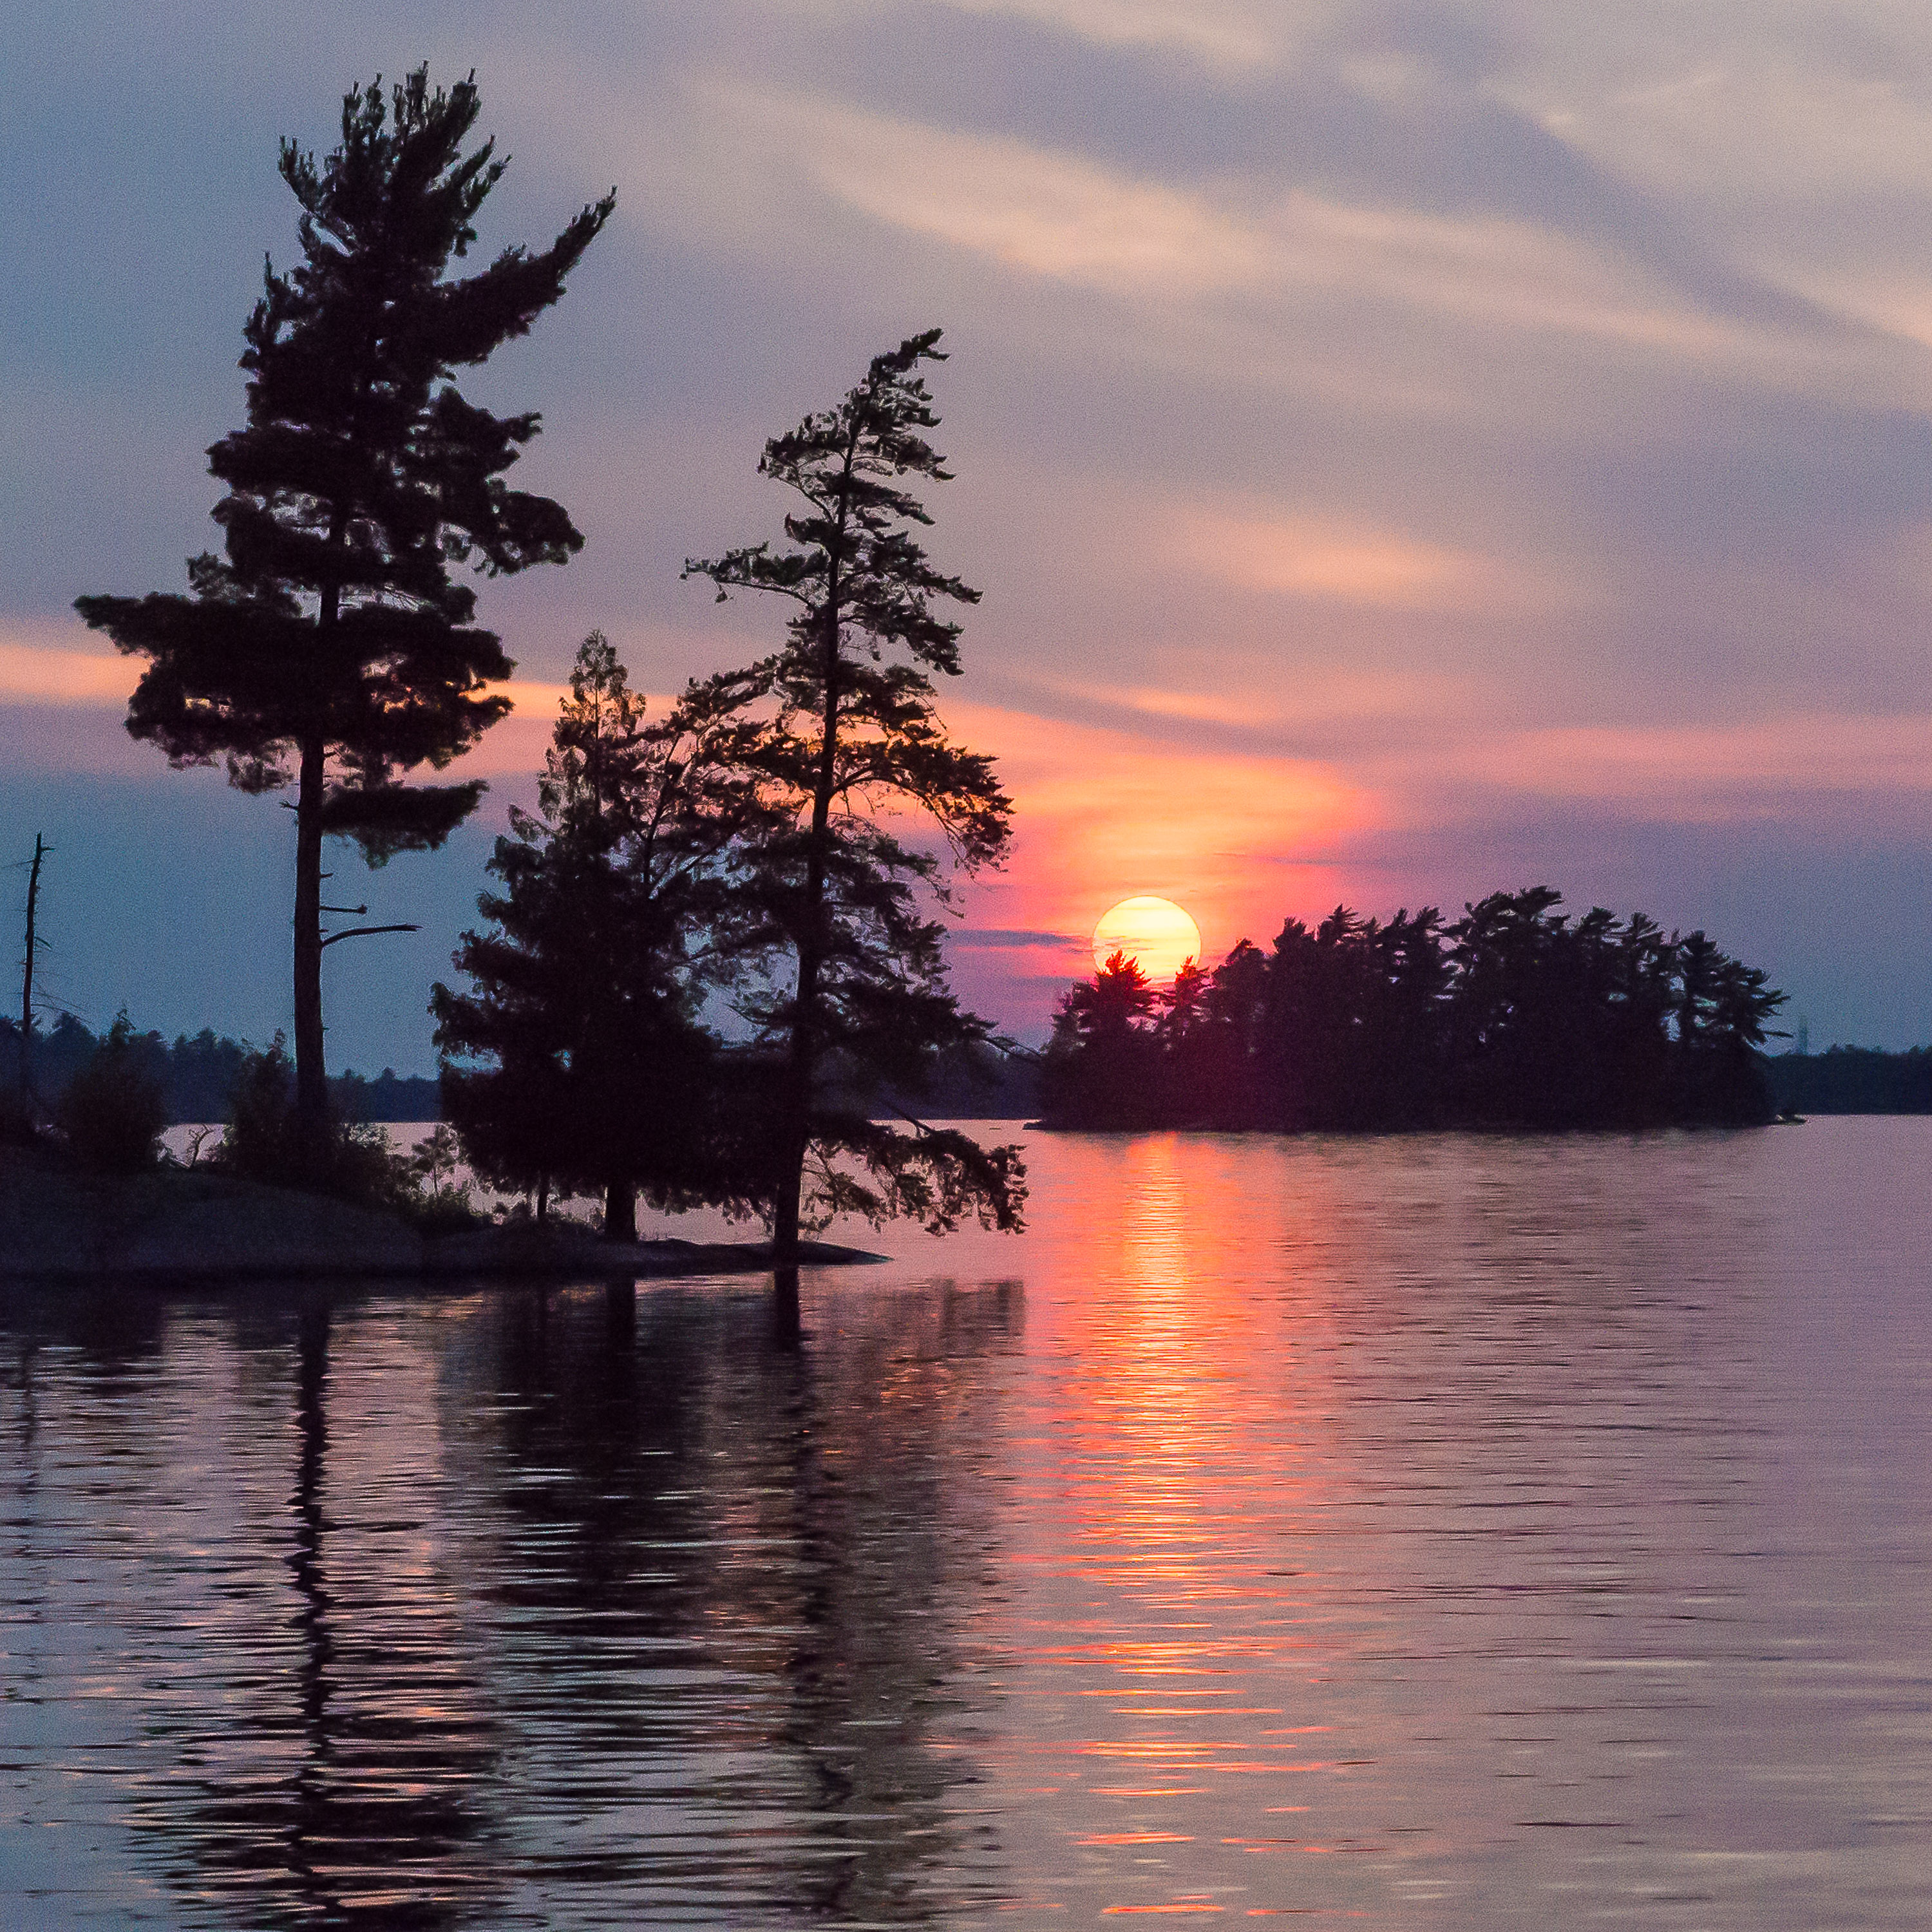
\includegraphics[width=\paperwidth]{FloodedSunset}}
\section{Discussion}
}

%%%%%%%%%1%%%%%%%%%2%%%%%%%%%3%%%%%%%%%4%%%%%%%%%5%%%%%%%%%6%%%%%%%%%7%%%%%%%%%8
% End of Document
%%%%%%%%%1%%%%%%%%%2%%%%%%%%%3%%%%%%%%%4%%%%%%%%%5%%%%%%%%%6%%%%%%%%%7%%%%%%%%%8

\end{document}
	
\end{frame}


